% Desarrollo
\chapter{Desarrollo} \label{chap:desarrollo}
	En este cap'itulo se describe de manera detallada todo el proceso de desarrollo de este proyecto de pasant'ia. Para ello, se va a describir c'omo fueron desarrolladas cada una de las fases involucradas.

\section{Fase 1: Preparaci'on Previa}
	Durante esta fase se realizaron diferentes reuniones organizadas por la tutora industrial con el fin de tener un entrenamiento en el software SAP. Para ello, distintos empleados de la compa\~n'ia estuvieron en dichas reuniones para dictar los talleres.
\newline
\newline
	Los talleres recibidos fueron acerca de los siguientes m'odulos: QM, MM, FI, CO y SD.
\indent Para cada m'odulo fueron explicados los conceptos b'asicos que est'an involucrados en cada uno. Espec'ificamente en el taller de Ventas y Distribuci'on, se explic'o el ciclo de ventas general. Para ello, la persona encargada, explic'o por detalle cada una de las etapas por las cuales pasa un proceso de ventas en general (Realizaci'on del Pedido de Ventas, Entrega, Facturaci'on). 
\newline
\newline
\indent Adicionalmente, fue impartido un taller sobre el lenguaje de Programaci'on ABAP/4, para conocer un poco acerca de la estructura del lenguaje. Durante este taller, se recibieron conocimientos acerca de: estructuras de control, herramientas que posee el lenguaje para emitir reportes. 
\newline
\newline
\indent Adem'as, se recibi'o material acerca de otro \textit{template} que fue desarrollado para otro tipo de industria, pero que sirvi'o como base para ver como el m'odulo de Ventas y Distribuci'on es puesto en pr'actica, y para servir como ejemplo a la hora de implantar dicho m'odulo a la empresa de bebidas de consumo masivo.
	
\section{Fase 2: Business Blueprint}
	Durante esta fase fueron desarrolladas las siguientes actividades:
\begin{itemize}
\item Identificar el proceso de Master Data (Datos Mestros) a desarrollar en SAP.
\item Identificar el proceso de Sales (Pedidos de Venta) a desarrollar en SAP.
\item Identificar el proceso de Shipping and Transportation (Embarque y transporte) a ser desarrollado en SAP.
\item Identificar el proceso de Billing (Facturaci'on) a ser desarrollado en SAP.
\end{itemize}

	Como fue explicado en el cap'itulo anterior, en esta fase se detallan cada uno de los procesos del negocio de la compa\~n'ia para la cual se est'a llevando el proyecto; esto involucra conocer los procesos actuales y como se podr'ian aplicar dichos procesos en SAP. 
\newline
\newline
\indent Para el caso de la empresa de bebidas de Consumo Masivo para la cual se est'a trabajando, se van a analizar cada uno de los procesos involucrados en Ventas y Distribuci'on, para ello, se proceder'a en los siguientes apartados a detallar cada una de las actividades mencionadas en la lista anterior.
	
\subsection{Identificaci'on del proceso de Master Data (Datos Maestros)}
	En esta actividad, los datos maestros que fueron estudiados e identificados para el caso de la empresa de bebidas de consumo masivo para la cual se est'a realizando esta configuraci'on, consistieron en los datos que forman parte de la estructura organizativa de la empresa. Para ello se realiz'o un estudio con otras empresas que manejan el mismo rubro para saber cu'al es el camino a seguir. 

	Para las Organizaciones de Ventas, se fijaron dos organizaciones para configurar en la siguiente etapa, y son las que se muestran en la siguiente lista:

\begin{itemize}

\item Nacional: Se va a encargar de atender a los clientes nacionales
\item Internacional : Se va a encargar de atender las exportaciones de los productos
\end{itemize}
	Luego se definieron los Canales de Distribuci'on. Para este caso, se decidi'o fijar 7 canales de distribución. Estos son los que se listan en la siguiente lista:

\begin{itemize}
\item Distribuci'on Directa: Este canal ser'a utilizado para atender a los clientes en general.
\item Intermediario: Este canal ser'a utilizado para atender a aquellos clientes que tengan alg'un intermediario con el que a trav'es de ellos realicen alguna compra de materiales.
\item Eventos: Este canal ser'a utilizado para captar clientes a trav'es de eventos que realice la compa\~nia. 
\item Institucionales: Esta canal ser'a empleado para atraer a clientes a trav'es de instituciones sin fines de lucro.
\item Mayoristas: Este canal ser'a empleado para atraer a aquellos clientes se compren al mayoreo.
\item Traslados: Este canal ser'a utilizado para aquellos clientes que est'en a lo largo del pa'is.
\item Exportaciones: Este canal ser'a utilizado para aquellos clientes que est'en en el exterior.
\end{itemize}
	A continuaci'on, se procedi'o a establecer los sectores en los cuales ser'an agrupados los materiales a producir, como se muestra a continuaci'on:
\begin{itemize}
\item Producto Terminado: Consiste en el grupo conformado por todas aquellas bebidas que vayan a ser vendidas por la empresa, que ya han sido elaboradas.
\item Otros: En este grupo entran aquellos materiales que fueron usados para la elaboraci'on de los productos finales, del cual qued'o un remanente.
\end{itemize}
	Como producto de esta primera etapa, en las Figuras ~\ref{fig:estructura1} y ~\ref{fig:estructura2} se muestra c'omo quedaron cada una de las unidades de la empresa estructuradas.
\begin{figure}[H]
\centering
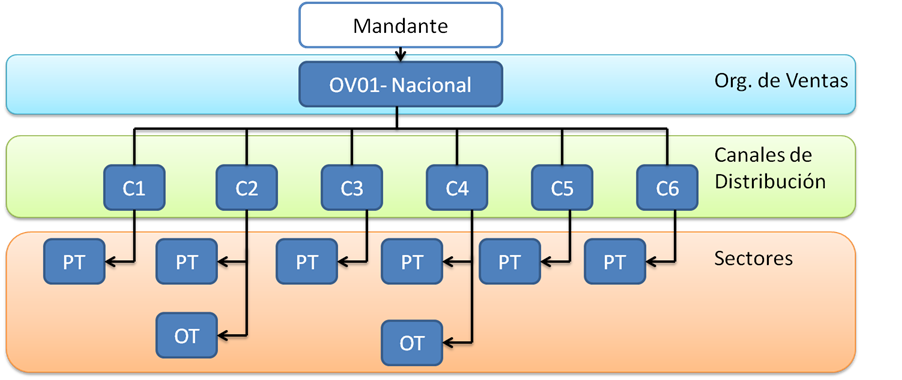
\includegraphics[scale=0.65,type=png,ext=.png,read=.png]{figures/Org1}
\caption{Estructura de SSA Beverage resultante de la Fase del Blueprint}
\label{fig:estructura1}
\end{figure}
\begin{figure}[H]
\centering
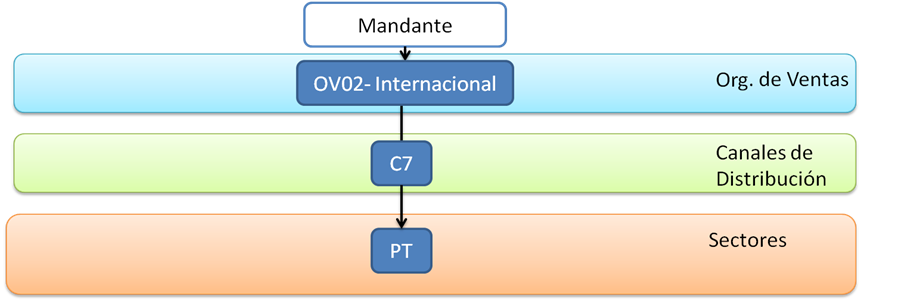
\includegraphics[scale=0.65,type=png,ext=.png,read=.png]{figures/Org2}
\caption{Estructura de SSA Beverage resultante de la Fase del Blueprint - Parte 2}
\label{fig:estructura2}
\end{figure}
Luego se procedi'o a establecer varias oficinas de ventas. Para esto, se decidi'o mantener la misma distribuci'on de los Centros de Distribuci'on que fueron colocados dentro del m'odulo de Gesti'on de Materiales (MM), en la cual se dividi'o al territorio en varias regiones. Luego, se defini'o una oficina por cada regi'on, quedando las mismas de la siguiente manera: Capital, Central, Los Llanos, Nororiental, Insular, Occidental, Andes y Zuliana.
\newline
\newline
	Posteriormente, se hizo la identificaci'on de los puestos de expedici'on por cada centro de distribuci'on. Dada la distribuci'on de las ofcinas de ventas en el p'arrafo anterior, y que las mismas presentan una distribuci'on equivalente a los Centros de Distribuci'on, se decidi'o establecer dos puestos de carga por cada uno, como se muestra a continuaci'on:
\begin{itemize}
\item Despacho: Este puesto se encarga de la entrega de los materiales a los clientes.
\item Retorno: Este puesto se encarga de recibir aquellos materiales que son enviados por los clientes, como por ejemplo: botellas retornables, etc.
\end{itemize}
	Para establecer los puestos de expedici'on en la siguiente etapa, fueron identificados dos puestos de carga por cada puesto de expedici'on.
\subsection{Identificaci'on del proceso de Sales (Pedidos de Ventas)}
	Dentro del proceso de ventas que es manejado por el m'odulo SD, este es el punto de partida, ya que el primer paso para poder realizar el ciclo de una venta de un material es la realizaci'on de un Pedido de Ventas. Para ello, es creado un documento de Pedido de Ventas que contiene varios tipos de informaci'on:
\begin{itemize}
\item Informaci'on personal del cliente
\item Informaci'on del(los) material(es) a adquirir
\item Informaci'on sobre las condiciones de pago
\end{itemize}
	Para ello, es necesario identificar varios puntos importantes en esta etapa:
\begin{itemize}
\item \textbf{Tipo de Pedido a realizar:} Representa el tipo de Documento a crear
\item \textbf{Clases de Mensajes:} Contiene las rutinas de impresi'on de documentos
\item \textbf{Tipos de Posici'on:} Cada rengl'on del documento relacionado con cada material representa una posici'on del documento
\item \textbf{Clases de condici'on:} Como su nombre lo indica, son condiciones. 'Estas son establecidas a los precios de los productos
\item \textbf{Esquemas de C'alculo:} Contiene las clases de Condici'on a utilizar
\end{itemize}
	Para este proyecto, se decidi'o copiar el Pedido Est'andar, el cual permite realizar un pedido normal, y as'i crear uno propio. Para las clases de mensajes se decidi'o adoptar la est'andar, al igual que los tipos de posici'on y las clases de condici'on, para crearlos posteriormente.
\subsection{Identificaci'on del proceso de Shipping and Transportation (Embarque y Transporte)}
	El segundo paso dentro del ciclo general de una venta en SAP es el proceso de Entrega (Shipping). Este consiste en generar un Documento de Entrega, en el cual consta, adem'as de los datos provenientes del Documento de Ventas al cual hace referencia, los datos relacionados con el puesto de expedici'on en el cual ser'a entregado el material solicitado. Para esto es necesario definir el tipo de Documento a utilizar. 
\newline
\newline
	Dado que en el segmento anterior se decidi'o definir un Pedido Est'andar, para esta parte del ciclo de Ventas se decidi'o definir un Documento de Entrega Est'andar, ya que es el que corresponde con el tipo de pedido establecido anteriormente.

\subsection{Identificaci'on del proceso de Billing (Facturaci'on)}
	El tercer y 'ultimo paso dentro del ciclo general de una venta en SAP es el proceso de Facturaci'on (Billing). Para este caso se define un tipo de documento de Facturaci'on acorde con el tipo de Pedido de Ventas y tipo de Entrega definidos anteriormente.
\newline
\newline
\indent Para el pedido Estandar definido m'as atr'as, fueron definidos dos tipos de Documentos de Facturaci'on: El primero, la Facturaci'on Est'andar, el cual es utilizado para crear la factura de un pedido existente, para as'i cerrar el ciclo normal de la venta de un material. El segundo, consiste en la \textbf{Anulaci'on de Factura}, 'este es usado para una vez que haya sido creada la factura de un pedido, y halla ocurrido alg'un problema durante el proceso en el cual fue realizado dicho pedido, el mismo se pueda anular, y as'i se pueda volver a crear.

\section{Fase 3: Realizaci'on (Construcci'on y Pruebas)}
	Las actividades desarrolladas en esta fase se dividieron en dos grupos principales: Configuraci'on Base del M'odulo de Ventas y Distribuci'on para SSA Beverage y Elaboraci'on de las facturas legales.
\newline
\newline
\indent A continuaci'on, se proceder'a a detallar cada uno de los dos grupos.
\subsection{Configuraci'on Base del M'odulo de Ventas y Distribuci'on para SSA Beverage}
	Para poder realizar las configuraciones, hubo que dividirlas en varios grupos, los cuales se muestran a continuaci'on:
\subsubsection{Configuraci'on de la parte organizativa de la Empresa}
	Este grupo fue compuesto por las configuraciones realizadas para definir la estructura de SSA Beverage. Para ello, se ingres'o a SAP, y a trav'es del Customizing, fue posible efectuarlas. Se comenz'o configurando las Organizaciones de Ventas (Ver Figura ~\ref{fig:organizaciones}, Canales de Distribuci'on (Ver Figura ~\ref{fig:canales}) , Sectores (Ver Figura ~\ref{fig:sectores}) , 'Areas de Ventas (Ver Figura ~\ref{fig:areas}) y Oficinas de Venta (Ver Figura ~\ref{fig:oficinas}).
\begin{figure}[H]
\centering
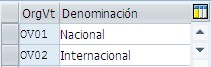
\includegraphics[scale=0.65,type=jpg,ext=.jpg,read=.jpg]{figures/OrgVentas}
\caption{Organizaciones de Ventas}
\label{fig:organizaciones}
\end{figure}
\begin{figure}[H]
\centering
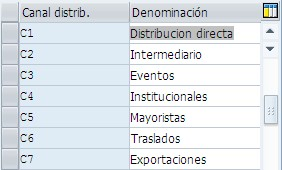
\includegraphics[scale=0.65,type=jpg,ext=.jpg,read=.jpg]{figures/CanalesDistribucion}
\caption{Canales de Distribuci'on}
\label{fig:canales}
\end{figure}
\begin{figure}[H]
\centering
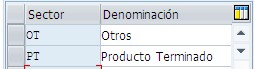
\includegraphics[scale=0.65,type=jpg,ext=.jpg,read=.jpg]{figures/Sectores}
\caption{Sectores}
\label{fig:sectores}
\end{figure}
\begin{figure}[H]
\centering
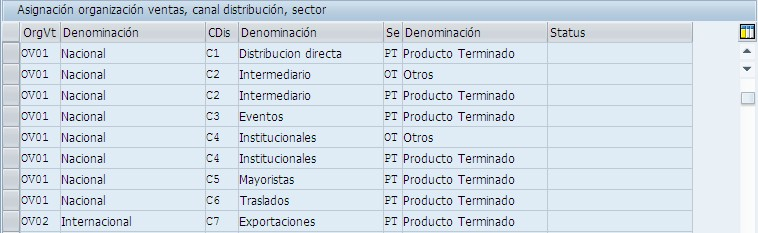
\includegraphics[scale=0.65,type=jpg,ext=.jpg,read=.jpg]{figures/AreaVentas}
\caption{'Areas de Ventas}
\label{fig:areas}
\end{figure}
\begin{figure}[H]
\centering
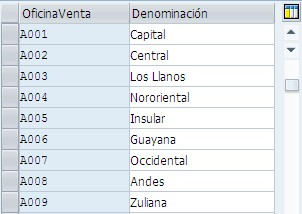
\includegraphics[scale=0.65,type=jpg,ext=.jpg,read=.jpg]{figures/OfVenta}
\caption{Oficinas de Ventas}
\label{fig:oficinas}
\end{figure}

	Luego, se procedi'o a realizar la configuraci'on de las unidades encargadas de la entrega de los materiales (Puestos de Expedici'on y Puestos de Carga). Para el primero se muestra la Figura ~\ref{fig:expedicion} que muestra los puestos de expedici'on definidos, y para el segundo, en la Figura ~\ref{fig:carga} se muestra parte de los puestos de carga creados.
\begin{figure}[H]
\centering
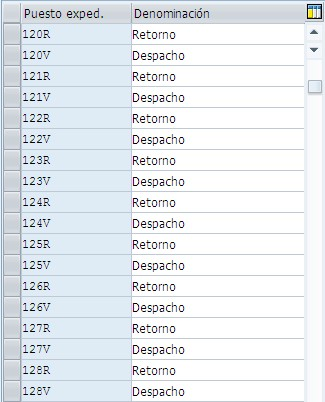
\includegraphics[scale=0.65,type=jpg,ext=.jpg,read=.jpg]{figures/PuestosExpedicion}
\caption{ Puestos de Expedici'on definidos para el M'odulo SD}
\label{fig:expedicion}
\end{figure}
\begin{figure}[H]
\centering
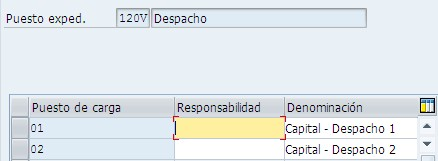
\includegraphics[scale=0.65,type=jpg,ext=.jpg,read=.jpg]{figures/PuestoCarga}
\caption{Parte de los Puestos de Carga definidos para el M'odulo SD}
\label{fig:carga}
\end{figure}
Despu'es que fueron creadas cada una de las unidades antes mencionadas dentro de SAP, las configuraciones posteriores consistieron en crear las relaciones entre las mismas. En la siguiente lista se muestra una lista con las configuraciones realizadas:
\begin{itemize}
\item Asignar las Organizaciones de Ventas creadas a la Sociedad
\item Asignar los Canales de Distribuci'on a las Organizaciones de Ventas
\item Asignar los Sectores a las Organizaciones de Ventas 
\item Asignar las Oficinas de Ventas a las 'Areas de Ventas
\item Asignar las Organizaciones de Ventas y Canales de Distribuci'on a los Centros de Distribuci'on
\item Asignar los Puestos de Expedici'on a los Centros de Distribuci'on
\end{itemize}
En las pr'oximas figuras se muestran las configuraciones realizadas.
\begin{figure}[H]
\centering
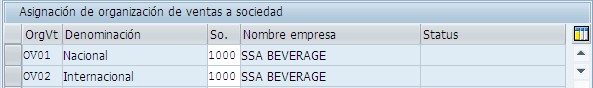
\includegraphics[scale=0.65,type=jpg,ext=.jpg,read=.jpg]{figures/OrgVentasSociedad}
\caption{Asignaci'on de las Organizaciones de Ventas a la sociedad Financiera}
\label{fig:asigna}
\end{figure}
	En la figura anterior se pueden visualizar las Organizaciones de Ventas creadas en las configuraciones anteriores asignadas a la Sociedad Financiera creada por el m'odulo FI. Dado que existe una 'unica sociedad financiera, lo que se hizo fue asignar las dos organizaciones a dicha sociedad.
\begin{figure}[H]
\centering
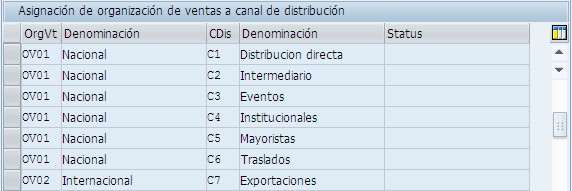
\includegraphics[scale=0.65,type=jpg,ext=.jpg,read=.jpg]{figures/OrgVentasCanales}
\caption{Asignaci'on de las Organizaciones de Ventas a los Canales de Distribuci'on}
\label{fig:asigna2}
\end{figure}
	En la figura anterior se puede visualizar la asignaci'on de las organizaciones de ventas a los canales de distribuci'on creados previamente. Para esto, previamente ya se habia establecido que los primeros seis canales iban a ser manejados por la Organizaci'on de Ventas \textbf{Nacional}, y que la Organizaci'on de Ventas \textbf{Internacional} iba a manejar el canal de Exportaci'on. 
\begin{figure}[H]
\centering
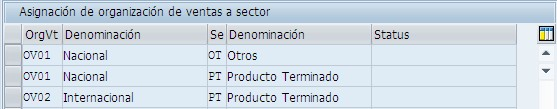
\includegraphics[scale=0.65,type=jpg,ext=.jpg,read=.jpg]{figures/OrgVentasSector}
\caption{Asignaci'on de las Organizaciones de Ventas a los Sectores}
\label{fig:asigna3}
\end{figure}
	En la figura anterior se puede ver la asignaci'on realizada de las Organizaciones de Venta a los Sectores. Esto permite que las organizaciones puedan manejar los materiales que vende de una forma organizada. Para la Organizaci'on de Ventas \textbf{Nacional}, se fij'o que estuviera asignada a los dos sectores definidos previamente (Producto Terminado y Otros). Por otro lado, la Organizaci'on de Ventas \textbf{Internacional} est'a asignada solo al segundo sector.
\begin{figure}[H]
\centering
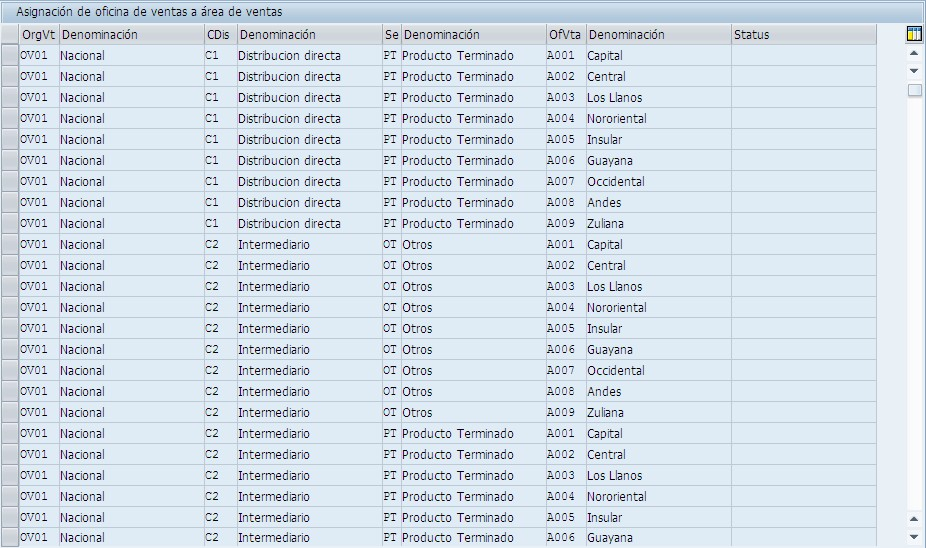
\includegraphics[scale=0.65,type=jpg,ext=.jpg,read=.jpg]{figures/OfVentaAreas}
\caption{Parte de la asignaci'on de las Oficinas de Ventas a las 'Areas de Ventas}
\label{fig:asigna4}
\end{figure}
	En la figura anterior se puede visualizar parte de la asignaci'on de las oficinas de ventas a las 'areas de ventas creadas anteriormente. Dado que fueron muchas, s'olo se muestra una parte de ellas. Lo que se quiso lograr con esto es asignar cada 'area con cada oficina, para que cada 'area de venta sea manejada por cada oficina creada.
\begin{figure}[H]
\centering
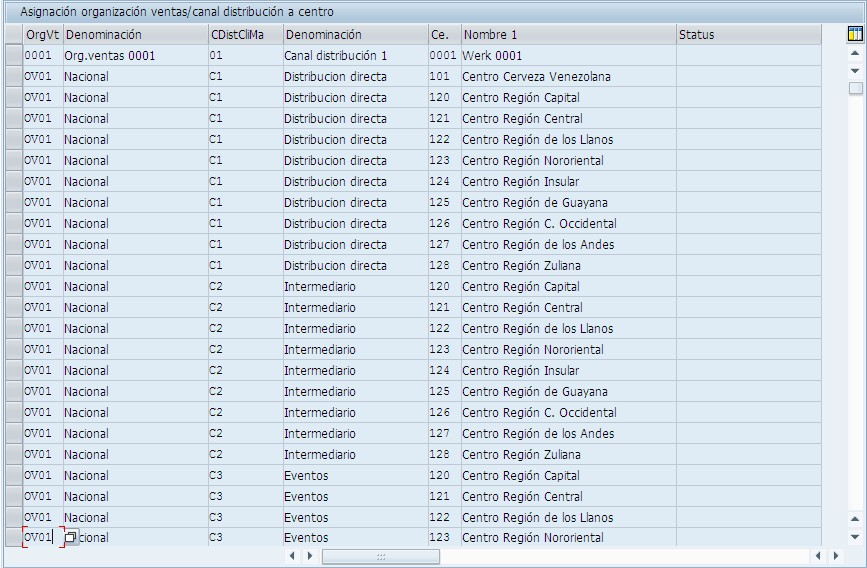
\includegraphics[scale=0.65,type=jpg,ext=.jpg,read=.jpg]{figures/OrgCanalCentro}
\caption{Parte de la asignaci'on de las Orgnanizaciones de Ventas y Canales de Distribuci'on a los Centros de Distribuci'on}
\label{fig:asigna5}
\end{figure}
	En la figura anterior se puede ver parte de la asignaci'on de las organizaciones de ventas y canales de distribuci'on a los centros de distribuci'on creados por el m'odulo MM. Aqui lo que se quiso lograr es que cada Organizaci'on de Venta con su canal de distribuci'on asociado a los distintos centros de distribuci'on creados previamente.
\begin{figure}[H]
\centering
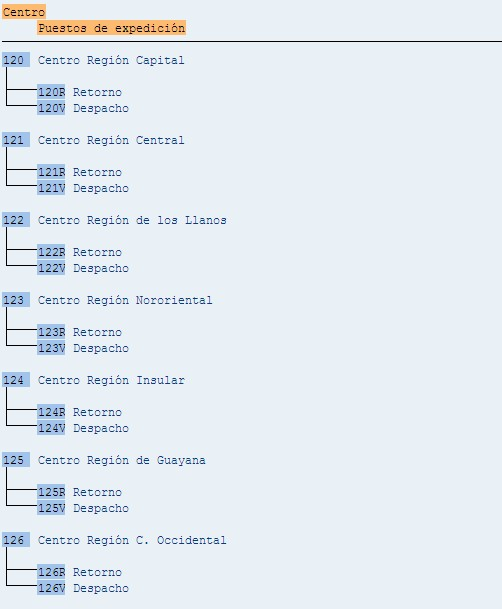
\includegraphics[scale=0.65,type=jpg,ext=.jpg,read=.jpg]{figures/ExpedicionCentro}
\caption{Parte de la asignaci'on de los Puestos de Expedici'on a los Centros de Distribuci'on}
\label{fig:asigna6}
\end{figure}
	En la figura anterior se puede apreciar parte de la asignaci'on de los puestos de expedici'on creados previamente, a los centros de distribuci'on configurados por el m'odulo MM. Lo que se quiso lograr es que cada centro de distribuci'on tenga dos puestos de expedici'on: Retorno y Despacho.

\subsection{Elaboraci'on de las Facturas Legales}
	Para el desarrollo de las Facturas Legales fue necesario el uso de los \textit{smartforms}, ya que los mismos producen formularios imprimibles. Para ello se tom'o como ejemplo un formulario est'andar ya existente en el sistema para hacer el dise\~no de uno propio. El mismo consta de varias partes bien diferenciadas:
\begin{itemize}
\item Pesos y Volumen: Contiene informaci'on sobre los pesos y vol'umenes totales de los materiales adquiridos.
\item Condiciones de Expedici'on y Pago: Contiene informaci'on sobre la forma en la cual se realiza la expedici'on y sobre la forma de pago.
\item Direcci'on del Cliente
\item Datos Generales: Contiene datos generales del cliente, como: n'umero del ciente, nombre, etc.
\item Posiciones de Factura: Contiene informaci'on detallada de cada material adquirido, como por ejemplo: N'umero de material, descripci'on, cantidad, precio unitario, etc.
\end{itemize}
	En la Figura  ~\ref{fig:facturas} se puede ver la factura que fue creada. En esta figura se pueden detallar varias partes bien diferenciadas:
\begin{enumerate}
\item En la parte superior se puede visualizar tanto el logo como el nombre de la empresa (SSA Beverage), as'i como su direcci'on y tel'efonos (Estos dos 'ultimos datos son ficticios, no son reales).
\item En el recuadro \textbf{Informaci'on de Pago}, se puede visualizar varios datos importantes: El n'umero y fecha de documento (N'umero de Factura generada por SAP y fecha de creaci'on de la misma), N'umero y fecha de la Nota de Entrega (N'umero de Entrega generado por SAP y fecha de la  creaci'on de la Entrega), N'umero y Fecha del Pedido (N'umero del Pedido de Venta generado por SAP y fecha de creaci'on de dicho pedido), N'umero  y Fecha de Referencia (N'umero del Pedido ingresado al momento de la creaci'on del mismo y la fecha de creaci'on del Pedido), N'umero del  Cliente (C'odigo del Cliente generado por SAP), Moneda (Moneda del documento) y el Importe de la Factura.
\item Del lado izquierdo al lado de dicho recuadro, aparecen los datos del cliente (Nombre y Direcci'on).
\item En el recuadro de \textbf{Condiciones} aparecen las condiciones de pago acordadas entre el cliente y la empresa, y la forma en como ser'a efectuada la entrega de los materiales.
\item  En el recuadro \textbf{Pesos - Vol'umenes} aparecen tanto el peso bruto como el peso neto total de todos los materiales adquiridos.
\item Finalmente en la parte inferior aparece detallado cada producto adquirido por el cliente. Para ello se presenta una tabla en donde se pueden ver las siguientes columnas:
\begin{itemize}
\item Posici'on: Posici'on del material en venta
\item Material: N'umero del Material generado por SAP
\item Denominaci'on: Breve descripci'on del material solicitado
\item Cantidad
\item Unidad: Unidad base en la que vienen los materiales
\end{itemize}
\item En el 'ultimo recuadro, aparecen dos montos: Importe de la Factura y Importe con derecho a descuento. El primero, es el monto total de la Factura. El segundo, es el monto sujeto a alg'un descuento (en caso de que pudiera aplicar)
\end{enumerate}
\begin{figure}[H]
\centering
\begin{tabular}{c}
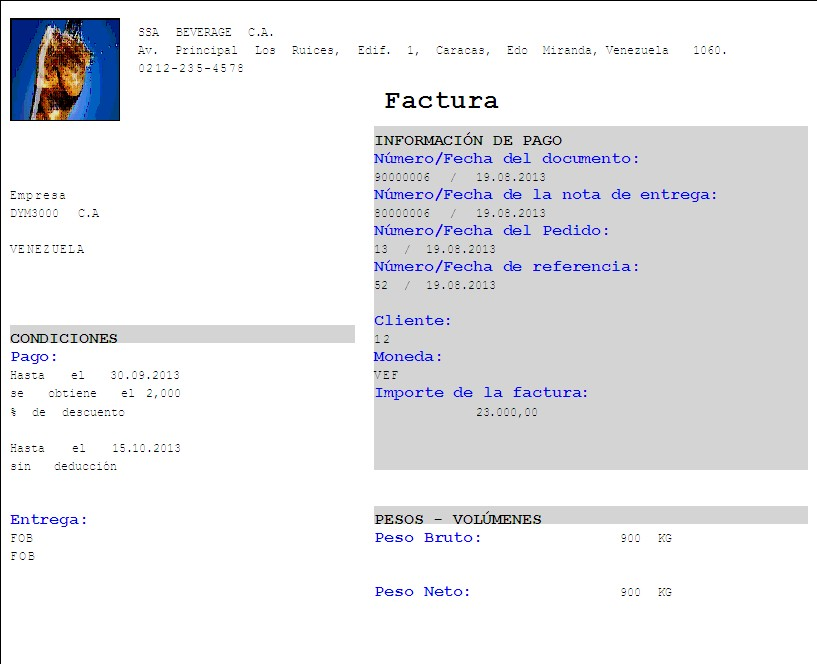
\includegraphics[scale=0.65,type=jpg,ext=.jpg,read=.jpg]{figures/Factura1}\\
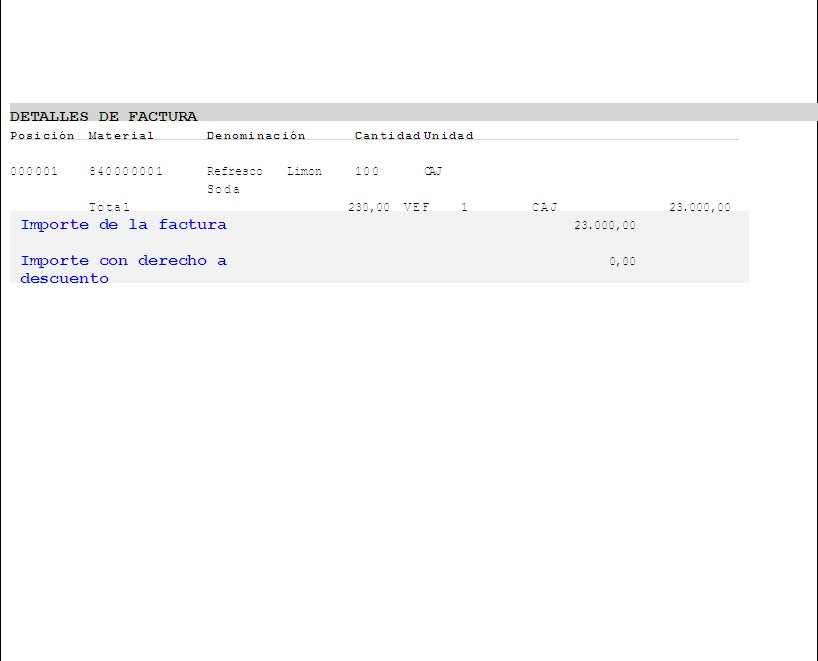
\includegraphics[scale=0.65,type=jpg,ext=.jpg,read=.jpg]{figures/Factura2}\\
\end{tabular}
\caption{Ejemplo de Factura creada para el m'odulo SD}
\label{fig:facturas}
\end{figure}

\subsection{Elaboraci'on del programa de Carga Masiva de Datos para el Maestro de Clientes}

\indent El Editor ABAP fue utilizado para el desarrollo del programa. Para esto, decidi'o modularizar el mismo. En otras palabras, el programa principal s'olo iba a contener el uso de variables y llamadas a procedimientos. 
\newline
\newline
\indent El primer paso para poder desarrollar este programa, fue el dise\~no estructurado del mismo. De tal manera que fue creado un Diagrama de Actividades siguiendo la notaci'on UML, con el fin de mostrar los pasos a realizar dentro del mismo. Para ello, se muestra dicho diagrama en la Figura ~\ref{fig:actividades}. 
\newline
\newline
\indent En dicho diagrama se puede visualizar el proceso general que sigue el programa. En primera instancia, se recibe el archivo, y se discrimina si es texto plano o si es de celdas (.xls), ya que en el segundo caso hay que realizar una conversi'on adicional dado que la funci'on est'andar de SAP que lee el archivo excel genera una estructura especial. Luego, mientras existan datos en la tabla, se procede a realizar la grabaci'on basada en la transacci'on XD01, la cual permite crear un nuevo registro en el maestro de clientes. Dicha grabaci'on se realiza con el fin de poder almacenar los datos en grupo, en vez de hacerlo de forma individual. 
\begin{figure}[H]
\centering
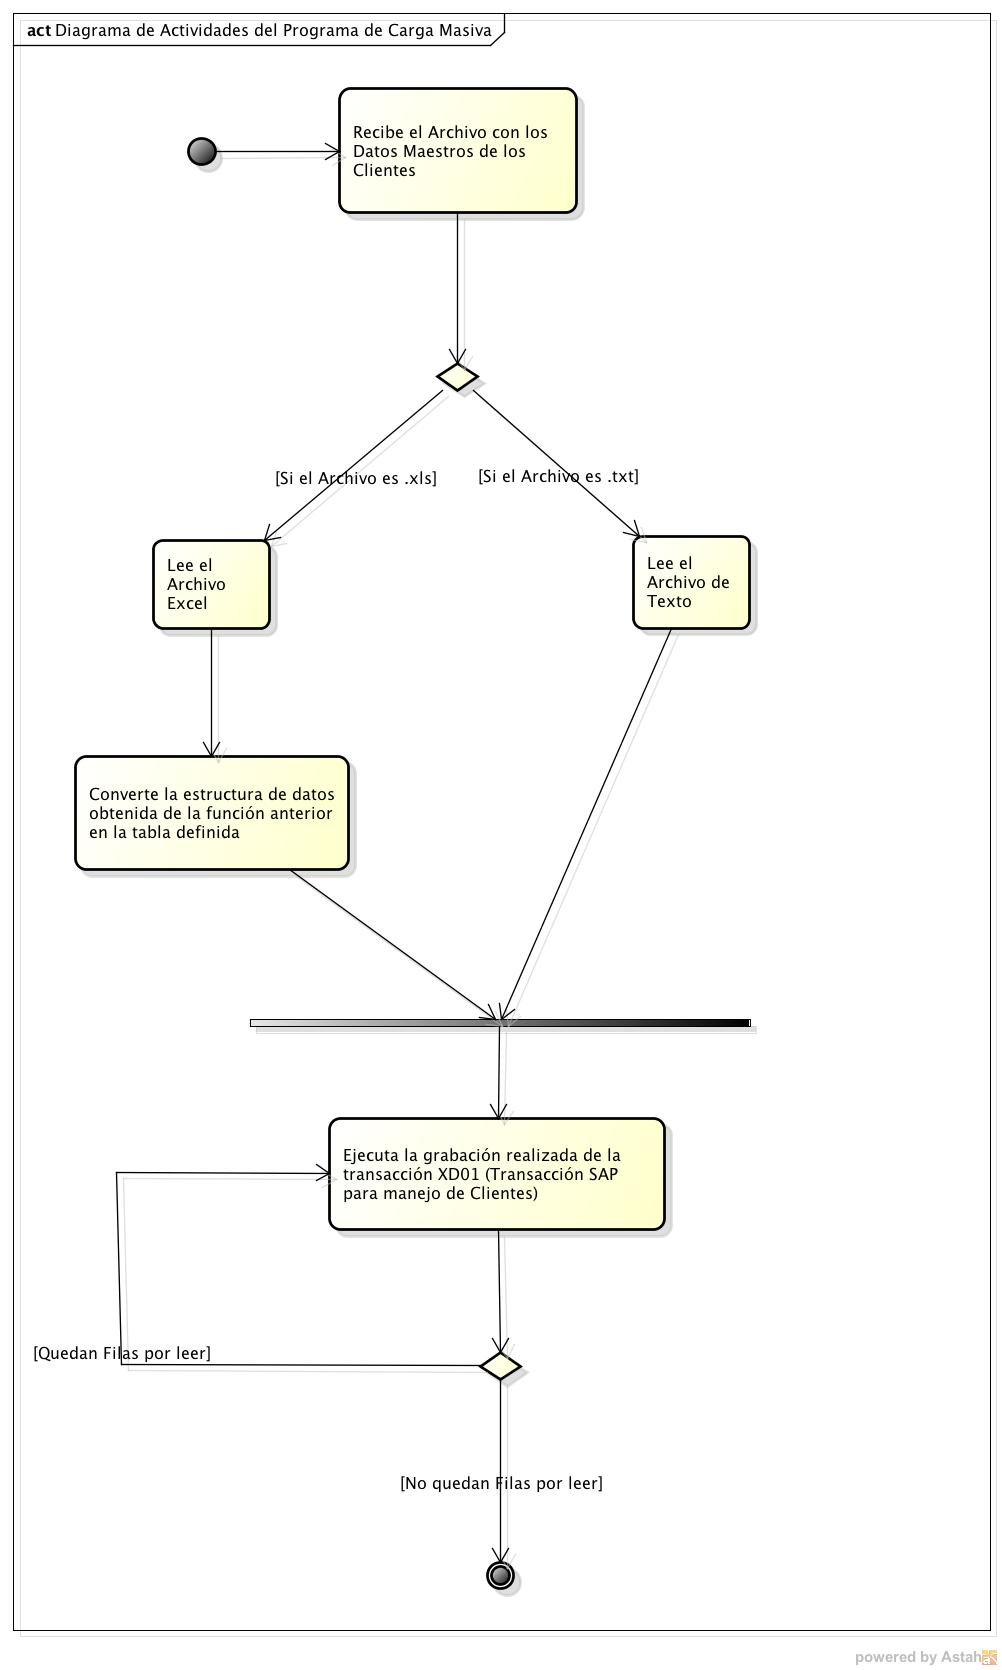
\includegraphics[scale=0.38,type=jpg,ext=.jpg,read=.jpg]{figures/DiagramaActividades}
\caption{Diagrama de Actividades del programa desarrollado en ABAP/4}
\label{fig:actividades}
\end{figure}
\indent Para poder lograr esto, fue necesario la creaci'on de dos \textit{Includes}: uno para la declaraci'on de variables, constantes, estructuras de datos, etc. Y otro, para la definici'on de funciones.
\newline
\newline
\indent Para poder recibir el archivo por pantalla, fue necesario el uso de los \textit{Selection Screens}, los cuales permiten colocar la direcci'on del archivo. En la figura ~\ref{fig:screen} se puede ver la pantalla inicial del programa de Carga Masiva, en el cual se le pide al usuario que introduzca la direcci'on del archivo. El usuario tiene la posibilidad de abrir un buscador de archivos tal y como sucede en cualquier otra aplicaci'on. Esto es posible gracias a la interfaz que posee SAP para estas actividades.
\newline
\newline
\begin{figure}[H]
\centering
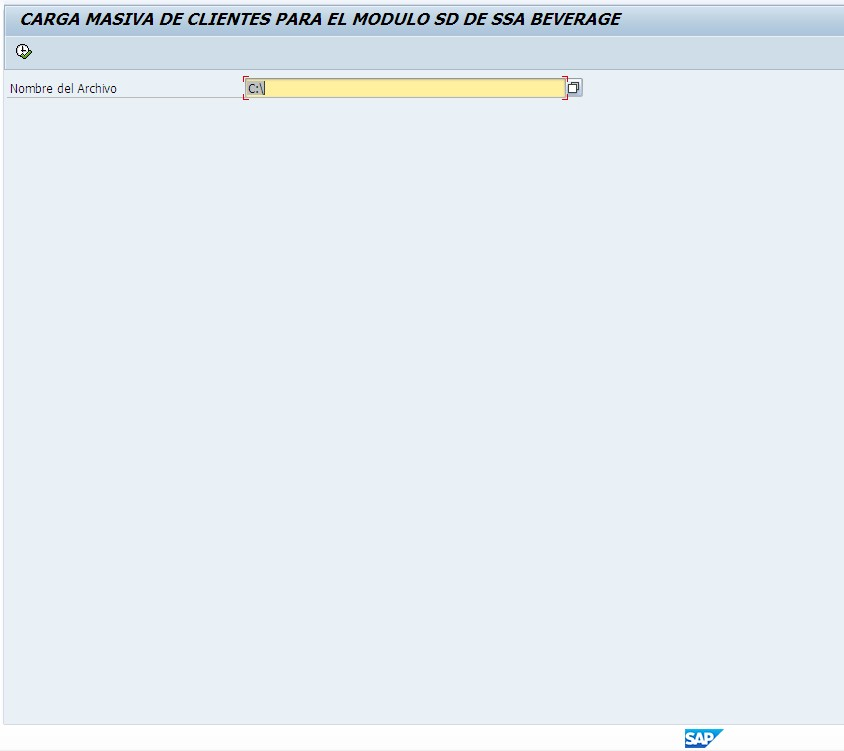
\includegraphics[scale=0.65,type=jpg,ext=.jpg,read=.jpg]{figures/screen}
\caption{Selection Screen para el Programa de Carga Masiva realizado}
\label{fig:screen}
\end{figure}
\indent La primera funci'on a implementar fue una que permitiera la lectura de un archivo en dos formatos: Texto Plano (.txt) y de Celdas (.xls o Excel como se le conoce comercialmente). En esta funci'on, se llama a una funci'on est'andar de SAP la cual permite leer un archivo en excel y transformar los datos a una estructura especial. Luego dicha estructura fue transformada a una estructura definida en uno de los \textit{Includes}. El proceso para un archivo plano fue an'alogo.
\newline
\newline
\begin{figure}[H]
\centering
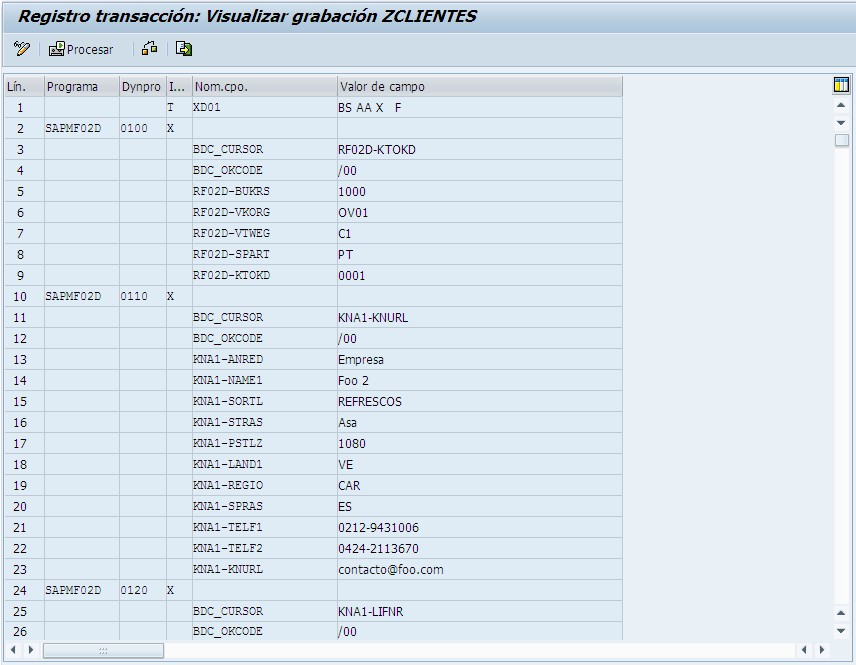
\includegraphics[scale=0.65,type=jpg,ext=.jpg,read=.jpg]{figures/sm35}
\caption{Grabaci'on realizada para la Carga Masiva}
\label{fig:sm35}
\end{figure}
\indent Luego se procedi'o a crear una grabaci'on para \textit{Batch Input} a trav'es de la transacci'on \textit{SM35}, con la cual, usando la transacci'on \textit{XD01} como base, se procedi'o a realizar la simulaci'on de la carga de datos. Luego, el c'odigo generado por dicha grabaci'on, fue utilizado dentro de otra funci'on creada para procesar los datos cargados anteriormente. De esta manera, se logra la carga masiva de datos en el Maestro de Clientes para el m'odulo de Ventas y Distribuci'on. En la figura ~\ref{fig:sm35} se puede ver parte de la grabaci'on realizada a trav'es de la transacci'on antes mencionada.


\section{Fase 4: Presentaci'on y Resultados Finales}
	Para la presentaci'on final en la empresa, el procedimiento a seguir fue la demostraci'on del ciclo est'andar que sigue el M'odulo SD (Pedido - Entrega - Facturaci'on). Para ello, se realiz'o un pedido, para luego continuar con la entrega y finalmente con la facturaci'on. En las Tablas ~\ref{tb:pedido} , ~\ref{tb:entrega} y ~\ref{tb:facturacion} se muestran los datos de prueba y los resultados obtenidos. 
	
\begin{table}[H]
\footnotesize
\scalebox{0.8} {
\begin{tabular}{l l l}
\toprule
\textbf{Nombre de la Transacci'on:} & VA01 &\\
\midrule
                 & \textbf{Clase de Pedido:} & ZSSA (Pedido Est'andar SSA Beverage) \\
                 \cmidrule{2-3}
                 & \textbf{Organizaci'on de Ventas:} & OV01 (Nacional) \\
                 \cmidrule{2-3}
                 & \textbf{Canal de Distribuci'on:} & C1 (Distribuci'on Directa) \\
                 \cmidrule{2-3}
                 & \textbf{Sector:}                   &   PT (Productos Terminados) \\
                 \cmidrule{2-3}
                 & \textbf{Pedido de Venta:}            & 21 \\
                 \cmidrule{2-3}
                 & \textbf{Solicitante:}              & 12 (DYM3000 C.A \\
                \cmidrule{2-3}
  \textbf{Datos de la Transacci'on:}              & \textbf{Dest. Mercanc'ia:}   &   12 (DYM3000 C.A \\
                 \cmidrule{2-3}
                 & \textbf{Nro. Pedido Cliente:} & 58      \\
                 \cmidrule{2-3}
                 & \textbf{Fecha de Pedido:} & 19.09.2013 \\
                 \cmidrule{2-3}
                 & \textbf{Bloqueo de Entrega:}  &      \\
                 \cmidrule{2-3}
                 & \textbf{Material:} & 84000001 (Refresco Lim'on Soda) \\
                 \cmidrule{2-3}
                 & \textbf{Cantidad de pedido} & 1 \\
                 \cmidrule{2-3}
                 & \textbf{Unidad de Pedido} & CAJ (Cajas) \\
                 \midrule
                 & \textbf{Resultado Obtenido:} & Exitoso \\
                 \cmidrule{2-3}
\textbf{Resultados de la Transacci'on:}    & \textbf{N'umero de Pedido arrojado por SAP:} & 00000021 \\
                 \cmidrule{2-3}
                 & \textbf{Observaciones:} &  \\
                 \bottomrule
\end{tabular}}
\caption{Proceso de Pedido de Venta presentado}
\label{tb:pedido}
\end{table}
	En la tabla anterior se puede apreciar el resultado de haber creado un Pedido de Ventas con los datos suministrados. Esto es, para poder iniciar el ciclo b'asico de ventas.
\begin{table}[H]
\footnotesize
\scalebox{0.8} {
\begin{tabular}{l l l}
\toprule
\textbf{Nombre de la Transacci'on:} & VL01N &\\
\midrule
                 & \textbf{Pedido:} & 00000021 \\
                 \cmidrule{2-3}
                 & \textbf{Puesto de Expedici'on:} & 120V (Despacho) \\
                 \cmidrule{2-3}
                 & \textbf{Centro de Distribuci'on:} & 120 (Regi'on Capital) \\
                 \cmidrule{2-3}
\textbf{Datos de la Transacci'on:}                  & \textbf{Almac'en:}                   &   PT01 \\
                 \cmidrule{2-3}
                 & \textbf{Cantidad Picking:}            & 1 \\
                 \cmidrule{2-3}
                 & \textbf{Unidad Picking:}              & CAJ (Cajas) \\
                 \midrule
                 & \textbf{Resultado Obtenido:} & Exitoso \\
                 \cmidrule{2-3}
\textbf{Resultados de la Transacci'on:}    & \textbf{N'umero de Entrega arrojado por SAP:} & 80000008 \\
                 \cmidrule{2-3}
                 & \textbf{Observaciones:} &  Para concluir la Entrega se procedi'o a Contabilizar \\
                 &                                      & el Material (Contabilizar SM) y fue exitoso\\
                 \bottomrule
\end{tabular}}
\caption{Proceso de Entrega presentado}
\label{tb:entrega}
\end{table}
	En la tabla anterior se puede ver el resultado de aplicar el segundo paso dentro del ciclo b'asico de la venta, el cual consiste en la creaci'on de una entrega con los datos suministrados. 
\begin{table}[H]
\footnotesize
\scalebox{0.8} {
\begin{tabular}{l l l}
\toprule
\textbf{Nombre de la Transacci'on:} & VF01 &\\
\midrule
                 & \textbf{N'umero de Documento:} &  80000008 \\
                 \cmidrule{2-3}
  \textbf{Datos de la Transacci'on:}                  & \textbf{Clase de Factura:} & Factura SSA Beverage \\
                 \midrule
                 & \textbf{Resultado Obtenido:} & Exitoso \\
                 \cmidrule{2-3}
\textbf{Resultados de la Transacci'on:}    & \textbf{N'umero de Factura arrojado por SAP:} & 90000007 \\
                 \cmidrule{2-3}
                 & \textbf{Observaciones:} &  Para concluir la Factura se procedi'o a Autorizar \\
                 &                                      & Contabilizaci'on (Esto es para crear Documento \\
                 &                                      & Contable) y fue exitoso\\
                 \bottomrule
\end{tabular}}
\caption{Proceso de Facturaci'on presentado}
\label{tb:facturacion}
\end{table}
	En la tabla anterior se puede visualizar el resultado de crear la factura para la entrega creada en el paso anterior. Con esto se concluy'o el ciclo b'asico de la venta dentro del m'odulo SD y con ello, la demostraci'on a la empresa.